\chapter{Fonony}

Mějme lineární řetěz stejných polarizovatelných molekul $A_1A_2A \cdots A_n$. Molekuly jsou fixované na svých pozicích.
Systém je při nulové teplotě, proto v mříži nebudou přítomny akustické fonony. Určte disperzní křivku  $\omega(k)$ a 
diskutuje chování $\omega(0)$ pro různé hodnoty $\alpha$. Pro molekulu $n$ máme zadánu pohybovou rovnici

\begin{equation} \label{Eq.phonons}
    \pdv[2]{p}{t} = -\omega_0^2 p + E \alpha \omega_0^2
\end{equation}

Rovnice \ref{Eq.phonons} je parciální diferenciální rovnice, kdy řešení budeme hledat v podobě rovinné vlny $p_n = p^* e^{i k x} e^{-i \omega t} = p^* e^{i (kx - \omega t)}$, kde $x = a . n$ je vzdálenost a $p^*$ amplituda.
Elektrické pole působíci na jednotlivou molekulu bude součtem příspěvků všech jejích sousedů. Sčítáme přes všechny páry tj. pro $m = n \pm 1, m = n \pm 2, \ldots$

\begin{multiline*}
    E_n = \sum_{m \neq n} E_{n,m} =  k_e  \sum \frac{2p_m}{d^3_{m,n}} = k_e \sum_{m \neq n} \frac{2 p^* e^{i k a m} e^{-i \omega t}}{a^3 |n - m|^3} \\
    = k_e \frac{2p^* e^{-\omega t}}{a^3} \sum \frac{e^{i k m}}{|n - m|^3}
\end{multiline*}

, kde $k_e = \frac{1}{4 \pi \epsilon_0}$, $d_{m, n} = a |m - n|$

Vyjádříme exponencielu pomocí trigonometrické funkce, z výrazu však nejdříve vytkneme $e^{i k a n }$

$$
    E_n = k_e  \frac{p^*e^{- i\omega t}}{a^3} e^{i k a n } \ldots
$$

Podle rady od cvičícího:

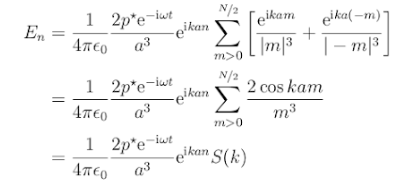
\includegraphics{Physics/trigon_exp.PNG}


Dosaíme li $E$ a tvar $p$ do pohybové rovnice dostaneme \ldots

$$
    \omega = \omega_0 \sqrt{ 1 - \frac{2}{a^3} k_e  \alpha S(k)}
$$

$$
    \omega_{k \to 0} = \omega_0 \left(  1  - k_e 2 \frac{\alpha}{a^3}  S(0)\right)
$$


